\documentclass[12pt]{article}

\usepackage{graphicx}
\usepackage{caption}
\usepackage[round]{natbib}
\usepackage{authblk}
\usepackage[utf8]{inputenc}
\usepackage{setspace}
\usepackage{rotating}
\usepackage[british]{datetime2}
\usepackage[hidelinks]{hyperref}
\usepackage{multicol}
\usepackage{wrapfig}
\usepackage[top=28truemm,bottom=26.5truemm,left=25.5truemm,right=25.5truemm]{geometry}

\renewcommand{\harvardurl}{\textbf{URL:} \url}

\renewcommand\Affilfont{\itshape\small}

\title{Dynamics of Armed Conflict Essay}
\author[1]{Marius Swane Wishman}
\affil[1]{Department of Sociology and Political Science, NTNU}

\date{\today}

\providecommand{\keywords}[1]
{
	\small	
	\textbf{\textit{Keywords---}} #1
}

\begin{document}

\maketitle

\begin{abstract}

\end{abstract}

\keywords{}

%tableofcontents
%\pagebreak

\onehalfspacing

\begin{multicols}{2}

\section{Introduction}

Growing literature on pre-colonial states and civil conflict. Disagreement on
the effects with regards to conflict.

This paper contributes to the literature by 1) presenting new data on
independent statehood in Africa. The data covers the 1800-1914 period and maps
an unprecedented number of independent states. 2) Finds that overall the
presence of pre-colonial states in Africa has had a conflict inducing effect
when looking at the total number of conflict related fatalities and number of
state-based violence events, in the post World War 2. 3) Finds that this
relationship only holds for high levels of pre-colonial state presence
\textit{some distance away from the current capital}\footnote{Roughly 100km},
while before that a negative relationship exists. This latter finding supports
the theory of `artificial states' that emphasises the problems associated with
founding states that correspond poorly to the underlying topography of
historical statehood. In areas where this correspondence is strong (areas with
high state presence, close to the capital) there is a consistent negative (with
varying significance) association with measures of conflict, while in areas
where modern states correspond poorly with the historical topography of
statehood (primarily areas with a rich history of independent statehood, on the
periphery of modern states) have experienced higher levels of conflict according
to my models/findings.

\section{Theory}

\subsection{Pre-colonial states}

Definitions and some none conflict findings. Discussion of the need to be aware
of not only if a given theory predicts peace or conflict, but also of where this
effects would take place.

\subsection{Conflict reducing}

\subsubsection{Internal monopoly of violence}

The \citet{Tilly1990} argument, States as stationary bandits gradually remove
internal competitors. Over time this reduces the number of actors within the
borders of a state that are able to wield organized forms of violence, and the
remaining ones' ability to do so. In the case of pre-colonial states, they are
now either once again `the' state (for example Morocco or Ashanti/Ghana), have
been incorporated into a larger state as part of its apparatus, or had its
institutions destroyed by some larger state (colonial or indigenous)
consolidating its role as the sole stationary bandit within its borders. In
other words within the former borders of a pre-colonial state there should be a
reduced number of potential wielders of organized violence (ceteris paribus)
depending on the pre-colonial states centralization/consolidation, itself a
product of time, reforms/political organization/idiosyncrasies and the proximity
to its capital. If the pre-colonial state was incorporated only partially into
the modern state, it could still pose a threat to the central state through
desertion (more on this later). If the pre-colonial state was destroyed, for
example by colonizers, without new state (colonial or post-colonial) entering
the resulting power vacuum other actors would do so, and become new stationary
bandits rivalling the state. How does this compare to other areas not formally
part of a pre-colonial state? These areas could inhabit roving bandits
\citep{Scott2009} or other actors already having filled an equivalent vacuum of
power. In other words, in this scenario pre-colonial state areas should be no
worse than other areas in terms of violence. Any resulting conflict running
through this mechanism should occur shortly after decolonization.

\subsubsection{Better Angles}

\citet{Pinker2012} builds an argument from cognitive science affective and
cognitive neuroscience, social and evolutionary  psychology, that humans are
capable of producing a lot of violence, but also show a lot of restraint and
compassion. It  all depends on the structures surrounding us, and how we are
socialised. He seeks to explain the extraordinary levels of
violence\footnote{\citet{Pinker2012} examines a number of forms of violence,
	both organized, unorganized, interpersonal, state based, international
and intra-national.} evident in the historical and archaeological record, and
its decline to modern levels.  Of relevance here, \citet{Pinker2012} identifies
five `trends' and five `historical forces' (as well as nine aspects of our
psychology, five promoting violence and four inhibiting it), that he uses
explain the observed decline in violence. The two first trends are the invention
of agriculture, the first cities and \textit{governments}. Early states
`pacified' their population following the logic of Hobbes Leviathan.  Leading to
an estimated fivefold reduction in likelihood of dying a violent death. Second,
the consolidation of large \textit{kingdoms with centralized authority} and an
infrastructure of commerce engaged their citizens in a `civilizing process',
whereby people were able to think and plan more long term.  This promoted acting
more rational (as \textit{homo economicus}) and inhibit impulsiveness to engage
in ever more positive sum games, leading to further reductions in violence at
individual, regional and country level. Again, the state (and increasing
commerce in this case) are the exogenous factor that sets the virtuous cycle in
motion. In addition, as polities become fewer and larger there is a reduction in
the number of actors that can engage in large scale/organized violence, leading
to fewer albeit bloodier conflicts. Nevertheless, the over all negative trend of
violent death continues. Partly as a result in the reduction in conflicts
outweigh their increased lethality, but partly also because of the reduction of
violence within polities. Citing \citet{richardson1960statistics}
\citet{Pinker2012} states that when area is held constant, there are far fewer
civil wars within borders than than there are interstate wars crossing them.
\citet{Pinker2012} also reiterates Tilly and Hobbes logic that ``As small
baronies and duchies coalesced into larger kingdoms, the centralized
authorities prevented them from warring with each other for the same reason that
they prevented individual citizens from warring with each other (and that
farmers prevent their livestock from killing each other): as far as an overlord
is concerned, private quarrels within his domain are a dead loss."

Of the `historical forces', the first is the `\textit{Leviathan}'; ``a state and
judiciary with a monopoly on the legitimate use of force, can defuse the
temptation of exploitative attack, inhibit the impulse for revenge and
circumvent the self-serving biases that make all parties believe they are on the
side of the angels." \citep[xxvi]{Pinker2012}. \citet{Pinker2012} goes as far as
concluding that the Leviathan ``may be the most consistent violence-reducer that
we have encountered in this book." \citep[680]{Pinker2012}. The contribution of
\citet{Pinker2012} is the synthesis of political and social science theories
with psychology. Critically, he shows that the self-control and aggression
reducing effects of the Leviathan can become habits so that citizens refrain
from violence ``Even when Leviathan's back is turned." \citep[681]{Pinker2012}. In
\citet{Pinker2012}'s eyes then, states, and the evolution of states have played
a big role in the historic decline of violence through shaping the environment
of its citizens to be more inducive to peace. If Pinker is right in thinking
that the formation and growth/expansion of states puts societies on a track
toward more peaceful societies, then areas with \textit{longer} and
\textit{deeper} histories of statehood should exhibit the effects of this, even
after 150-200 years. Working through the mechanisms of the interplay between
Leviathan and `gentle commerce', internalising or habitualising and perhaps
institutional inheritance (governance evolves so that areas that had some
governance in the past have better governance today).

\subsubsection{Conflict resolving institutions}

\citet{Wig2016} argues that ethnic groups with ties to pre-colonial statehood
are more likely to have inherited institutions that allow the ethnic group to
punish defections and hold their leaders accountable.  In this way, ethnic
groups with ties to pre-colonial statehood are better able to make credible
commitments, than 'non-state' ethnic groups.  Credible commitments help such
groups both prevent conflict from occurring in the first place, but also make
them better able to end conflicts when then they have broken out.  Empirically
\citet{Wig2016} finds that groups with histories of statehood do indeed
experience less dyadic conflict with their government.
\citet{Depetris-Chauvin2016} makes a similar argument and finds that regions
with exposure to pre-colonial statehood are more peaceful, \textit{ceteris
paribus}.

Inherited pre-colonial institutions could also provide specialised conflict
resolution institutions that allow local conflicts to deescalate, be resolved
before escalating to violence or channeled into non-violent processes of
redress. *** Need examples ***

\subsubsection{Hypotheses}

If one assumes that pre-colonial state presence is positively correlated with
post-independence state presence, then both the leviathan/pacifying
(\citet{Tilly1990} and \citet{Pinker2012}) and civilising \citep{Pinker2012}
mechanisms predict less violence in high state presence areas. Similarly higher
levels of pre-colonial state presence should increase the presence of conflict
resolving institutions or at least 'traditional leaders' how are better able to
make credible commitments. Thus, \citet{Wig2016} and
\citet{Depetris-Chauvin2016} also indicate the following hypothesis.

H1: Grid cells with higher levels of state presence, experience less civil
conflict (fatalities and onsets).\footnote{An interesting follow up, which would
	be true to Pinker's hypothesis would be to test against violent crime
	and homicides rates as well. For now at least that falls outside the
	scope of this paper, and as far as I am aware there is limited geo-coded
data available on this for Africa.}

Leviathan x gentile commerce. \textit{proxied} by higher levels of development
in areas of higher state presence. Predicts lower levels of violence in areas of
higher state presence, working \textit{through} development. This could be
tested using mediation analysis.

H1.1: Grid cells with higher levels of state presence, experience less civil
conflict mediated by higher levels of economic development.

Habitation/internalisation predicts lower levels of violence in higher state
presence areas \textit{contingent} on \textit{continuation} of state presence,
as this is quickly `unlearned'. In Africa this is almost exclusively central
(historical) Ethiopia and perhaps parts of South Africa depending on the
definition of continuation. However, a global sample would be interesting and
perhaps contribute new insights to the argument that colonialism caused much of
the woes and conflicts in the non-western world.


\subsection{Conflict inducing}

\subsection{Symbols of past sovereignty}

Following the innovation and spread of nationalism as an ideology, past
independence and glory (real or imagined) became an important ingredient in any
struggle for national independence. And as the current international system of
inviolable international boundaries between formally equally sovereign states
took shape following the World Wars, past violations of sovereignty added
further to the potential of past states to provide the basis for ethnic claim
making \citep{Ahram2019, Shelef2016}. 

Beyond formal claims to the right to self determination past states can provide
symbols that conflict entrepreneurs can use to overcome collective action
problems and mobilise for conflict. In recent years a number of Islamic groups
in North and West Africa have referred to various 1800s Islamic states either as
a namesake, such as the Macina Liberation Front, or stated inspiration in the
case of the Movement for Oneness and Jihad in West Africa (MUJWA) and the
Vanguard for the Protection of Muslims in Black Africa (Ansaru), who seek or
claim to revive the jihads of the Tokolor and Sokoto Empires respectively
\citep{Zenn2015}. However, the phenomenon is clearly not limited to Islamist
groups. For example, the Cyraneica Liberation Army refers to a short lived
kingdom in Eastern Libya, and elected a descendent of the former king as their
leader \citep{Ahram2019}. Further examples include the various Afrikaaner groups
aiming to reestablish the Boer Republics in South Africa.

\subsection{Networks useful for insurgency}

In addition to symbols, pre-colonial states can leave behind formal and informal
social networks that lower the cost of insurgent collective action
\citep{Wig2016, Wood2000}. The most visible examples of this are cases in which
kingdoms were ruled indirectly and remained intact into the modern era. Examples
include: Buganda, a relatively centralised kingdom in Uganda that led a brief
and unsuccessful rebellion against the Obote regime \citep{Tuck2005}, the Mwati
of the pre-colonial-come-traditional kingdom Lunda-Yeke in the Democratic
Republic of Congo attempted the secession of the Katanga region following the
independence of Zaire, and the sultan of Aussa (Awsa) violently resisted the
Ethiopian Dirge regimes attempt to depose him. While his Afar (ethnic group)
Liberation Front did not achieve independence, the institution of the sultanate
survived to this day \citep{Shehim1985, Hanfare2011}.

Other kingdoms were formally disbanded, but nevertheless were able to retain
regional elite networks, as exemplified by the aforementioned Al Senussi
dynasty/clan/tribe in Cyraneica who mobilised on a mix of resentment among the
population that they had received an unfair share of Libya's oil wealth (largely
stemming from wells in the region), the increasing frustration with the
Tripoli government following the toppling of Muammar Gaddafi and allegedly
elites who had prospered under the former monarchy \citep{Fetouri2012}.

The longer and stronger the recent history of independent statehood, the
stronger the symbolic value and legal claims based on that history would be.
Equally, the more likely networks (formal or informal) are to have survived. If
these factors are indeed conflict inducing, then the following hypothesis should
be true:

H2: Grid cells with higher pre-colonial state presence experience higher levels
of civil conflict. 

\subsubsection{Central State Weakness/Collapse}

When modern states `collapse' or in another sense achieve `failed state' status,
it creates a (series of) power vacuums and room/need for other actors to fill
the various roles usually filled by the state. At the regional level one can
imagine a handful of actors capable of filling this vacuum (of power and
service provision), one of which is pre-colonial state. Other candidates could
be active rebel groups, religious organizations and ethnic groups (not tied to
pre-colonial states). I would argue that pre-colonial states and active rebel
groups have distinct advantages above the others. Prime mover advantage and
capacity to monopolise violence on part of rebel groups, and legitimacy and
organizational benefits on the part of pre-colonial states.

The dynamics of this lie in how state collapse unfolds and `evolves'. Although I
am not sure if I will be able to test or properly examine this process I will
nevertheless sketch out how I imagine it (typically) unfolds.

Democratic collapse, succession/reform crises, state predation and/or civil war
are usually on the path toward state failure\citep{Goldstone_2008}. Once a state
has failed, lost its legitimacy and effectiveness \citep{Goldstone_2008}, other
actors will attempt to fill the void. This happens at all levels of government I
imagine, but most visibly at the country (repeated coups, attempts to overthrow
the government) and regional level (various forms of regional self governance).
I will focus on pre-colonial states reemerging as a basis of regional self
governance  (RSG) and the dynamics of it. If or when a pre-colonial state,
through either ethnic group, formal institutions or less formal networks, begins
to engage in RSG it sets out on a path that will at some point clash with the
interests of the central government. Because of its position as a pre-colonial
\textit{state} it is inevitably a challenge to the integrity of the state as a
whole. This creates a potential for further conflict, along new lines, in often
war torn countries. 

A different aspect of pre-colonial states engaging in RSG is that they can
create pockets of relatively functioning government within otherwise failed
states. I believe this can at least be tentatively explored on few case-by-case
basis using the data I have available. Do areas of high state presence (see data
section) outside the capital, experience a drop in combat events after engaging
in RSG. 

The example I primarily had in mind is  Puntland in Somaila, which corresponds
to the pre-colonial state of the Majarteen sultanate, has engaged in RSG as an
autonomous state within Somailas federal system. In terms of both peace and
prosperity the region has fared better than the rest of Somalia. Unlike
Somaliland the state is not seeking full independence. However, they do have
their own military forcer and tensions could rise if the central government were
to attempt further integration.

Other potential cases in Africa (see data) include Chad, Nigeria, DRC,
Sudan/Darfur and Lebanon.

Consider the illustrative case of the Russian federal state of Tatarstan. The
Tatar Khanate of Kazan was conquered by Ivan the Terrible in 1552 and
incorporated into the Russian empire as Kazan province by Peter the Great in
1708 \citep{Sharifzhanov_2007}. Despite Russification policies until the reign
of Cathrine II the Great (1762-96), when the Russian Empire collapsed following
the February revolution of 1917 Tatar nationalist seized the moment and declared
the creation Idel-Ural state \citep{Devlet_1993}. The nascent state laid claim
to boundaries closely resembling those of the old Khanate \citep{Hartley2020},
but the Bolsheviks and the Red Army were able to thwart the secession after a
month \citep{Hartley2020}. While the Tatars of Kazan no doubt were able to
retained their dreams of independence in large part to the ethnic and religious
differences between themselves and their rulers, it is striking that the
proposed borders follow those of the old Khanate and not of settlement patterns
of the Tatar ethnic group who were spread over a larger territory as part of the
Russification policy of the Tsars. Part of the movements goals was also the also
to allow Tatars émigré populations to return to their homeland
\citep{Devlet_1993}. When in turn the Soviet Union began to open up and collapse
in 1990-1991, the space once again opened up for the Tatars to reassert their
sovereignty. Following the example of Moscow and Russia the Tatar Autonomous
Soviet Socialist Republic declared itself a sovereign republic within the USSR,
which it attained in a declaration adopted by the Supreme Soviet. Thus on 12
June 1991 Russia acquired two presidents, Boris Yeltsin and Mintimir Sheymiev
\citep{Sharifzhanov_2007}. A referendum was set for 21 March 1992 on the
question of Tatarstan's independence. Authorities in Moscow tried to prevent
the referendum through the Constitutional Court of Russia and televised appeal
by Yeltsin to boycott the referendum, warning that an affirmative response
``would possibly lead to bloodshed." \citep{Sharifzhanov_2007}.  Nevertheless,
the referendum went ahead in the presence of international observers and boasted
a turnout 82 percent of which 61.4 percent voted for independence
\citep{Devlet_1993}. Following the referendum a new constitution was drafted
confirming Tatarstan's sovereignty. ``The Republic of Tatarstan shall be a
sovereign state, a subject of international law, associated to the Russian
Federation - Russia - on the basis of the Treaty on Mutual Delegation of Powers
and Subjects under Jurisdiction." \citet{Sharifzhanov_2007}. Unlike Chechen
leaders the Tatar leaders did not threaten use violent resistance to secede from
Russia, and through negotiations with the Yeltsin government they were able to
carve out a unique position of autonomy within the Russian Federation in 1994.
The different positions on the use of violence between the Chechens and Tatars
I believe is due to the feasibility of armed resistance to even a greatly
weakened Russian state based on geographic conditions. Chechnya is on the very
edge of the Russian periphery and is a mountainous country. Tatarstan on the
other hand lies relatively close to Moscow, and its steppe terrain lends an
advantage to modern national armies. In the words of the Chairman of the
Tatarstan parliament: ``We take a completely \textit{realistic} view of the
state of affairs: full independence is too abstract and unnecessary a concept
whereas Tatarstan and Russia are linked by inseparable bonds."
\citep{Sharifzhanov_2007}(emphasis added). At the same time parallels were still
drawn all the way back to the Kazan Khanate. During a speech at the first World
Congress of Tatars the Tatarstan president Mintimir Sheymiev declared that:

\textit{The history of the Tatars nation is very difficult and tragic. The
Tatars lost their Bulgar state, but found a respectable place for themselves
within the Golden Horde. After its collapse they created the khanates of Kazan
[...] the restoration of statehood was an idea ever present in Tatar history.}
(cited in \citet{mustafin1995pervyi}, 113).

H2.1: Grid cells with higher state presence experience higher levels of civil
conflict following state collapse. 

Currently not testing this hypothesis for a lack of a good measure of state
collapse. Of course, this is not insurmountable, but I am not sure if it
falls outside the scope of this paper. Perhaps this is best proxied by resent
decolonisation/independence in the African context, which is somewhat testable
by running the models of sub-samples of years. Specifically compare 1946-69 (or
so) to other subsets of years. Perhaps split by decades. This would of course
be an instance of state weakness more than collapse (unless you count it as the
collapse of the colonial regime, in which case it is apt).

\subsubsection{Political Inequality}

In countries where an ethnic group has a history of statecraft, said group is
likely to be have an over sized share of power in government. This can come
about through indirect colonial rule, which preferred to leave existing power
structures intact, or by seizure from less politically experienced groups
following independence \citep{Paine2019}. \citet{Paine2019} argues that such
state groups are likely to either exclude other groups from power, leaving them
with few options outside violence to achieve political representation. Or, in
the cases where state groups are are excluded themselves, they have the means to
organize and solve the necessary collective action problems and will reclaim
their dominating position by force \citep{Paine2019}. In case of fighting then,
it would happen in the area of the state group only in the cases where that
group was excluded from power. However, using our more fine grained data it is
apparent that this is far more common than \citet{Paine2019} supposes.

%TODO: find the mean number of different pre-colonial states per country from
%the HSE analysis

In \citet{Paine2019}'s data there are no instances of multiple state groups in
one country, and so he does not account for this in his theory. However, in our
more exhaustive data this occurs in several countries. Following
\citet{Paine2019}'s logic however, it would be expected that only one of the
groups were handed (or grabbed) the keys to the kingdom following independence,
and that other state group(s) would be relatively more likely to challenge any
attempts at exclusion.  As this is a continuation of \citet{Paine2019}'s
original mechanism, this would also be best proxied by high levels of state
presence far from the capital predicting higher levels of violence.

TODO: where does this predict conflict, and how to best test it. 

\subsubsection{Resistance to western influence}

An interesting hypothesis proposed by \citet{Wishman} builds on the finding that
where European colonizers met organized/powerful states (often Muslim), they
more often either took longer to colonise them or not at all, if/when they did
they were integrated more indirectly \citep{Gerring2011, Hariri2012,
Englebert2000}. This left these areas more isolated from western influences,
particularly that of protestant missionaries \citep{Woodberry2012}. If so, areas
of higher states presence should have been exposed to less western influences
such as humanism, `the escalator of reason' \citep{Pinker2012} and democracy
\citep{Woodberry2012, Hariri2012}, leading to less democratic and peaceful
outcomes in the post-colonial period \citep{Hegre2006}

H2.2 Grid cells with higher levels of state presence, experience more civil
conflict mediated by lower levels of support for humanist ideas, liberal
values or democracy.

Currently not testing due to lack of data.

\subsection{Conflict regulating}

Both sides to the existing literature could be right if there is some
intervening variable that causes state presence to be conflict inducing in one
instance and conflict reducing in another instance. I propose/present two
candidates for such an intervening variable.

\subsubsection{Artificial states}

Within the literature there are a number of conceptualisation and definitions of
`artificial states' or states whose borders are more or less `artificial'
\citep{Alesina2011, Clapham1996, Englebert2002, Herbst2014}. The underlying
principle, I argue, is the degree to which current states conform to the
pre-existing topography of historical statehood (which is itself a product of
geography and the military/political reach of political entities). The measure
of pre-colonial state presence presented below captures this better than
existing measures (such as the straightness of boundaries \citep{Alesina2011} or
the variance in pre-colonial ethnic centralisation \citep{Englebert2002}). The
only caveat is that it does not distinguish between the presence of for example
the pre-colonial Tunisian state, who the current country of Tunisia corresponds
very well with, or the kingdom of Darfur, who does not correspond to any current
country. To illustrate how the pre-colonial state presence can measure state
artifice, take the case of Ethiopia. Ethiopia contains a clear continuation of
the pre-colonial (in terms of time period) Empire of Ethiopia, but it also
contains a number of other pre-colonial states (conquered by the Ethiopian
Empire in the period cover in our data). In this example high levels of state
presence would most often reflect a strong presence of the Ethiopian state and
thus, for as long as its still inside the boundary of modern day Ethiopia, it
would indicate low state artifice (or natural borders). However, The further
away from the capital one would go the less likely and the less strong is this
presence, and equally the more artificial it is if this is part of Ethiopia
today. Additionally, if one is far from the capital and yet there are high
levels of state presence, it most likely represents the presence of one of the
kingdoms most recently incorporated into the Ethiopian Empire (such as the
aforementioned sultanate of Aussa). In this area high values would also indicate
a poor conformity to the existing history of statehood, and thus be more
artificial.  Likewise, areas of little to no pre-colonial state presence close
to its current capital would indicate a state built without any precedent or on
top of colonial institution, and thus also be more artificial. The literature
suggest that artificial states experience more conflict 
\citep{Alesina2011, Englebert2002}, which implies the following hypotheses:

H3: The relationship between grid cell level levels of state presence and civil
conflict is modified by the grid cell's distance to the current capital (as
measured by an interaction term).

H3.1: Grid cells with higher levels of state presence, further from the current capital 
experience higher levels of civil conflict.

H3.2:  Grid cells with higher levels of state presence, closer to the current capital 
experience lower levels of civil conflict.

\subsubsection{Multiple pre-colonial states}

It could be true as that pre-colonial states are individually (or dyadically)
conflict reducing \citep{Pinker2012, Wig2016}, but as the number of groups with
ties to pre-colonial states increase this positive (normatively speaking)
relationship breaks down due to increased complexity of bargaining
\citep{Walter2009} and altered incentives for the state to punish (rather than
accommodate) early groups who (try or threaten to) assert autonomy in order to
dissuade others from doing the same. This is one of the arguments of
\citet{Wishman}, but has only been tested at a country level (albeit on a global
sample), but found that countries that were hosts to more historical state
entities (pre-colonial states in this paper), experienced more civil conflict in
the post World War 2 period. If the observed correlation is due to any of the
mechanisms that the authors outline, then there should be an equivalent
correlation between areas of high state presence in countries with multiple
pre-colonial states.

H4: The relationship between grid cell level levels of state presence and civil
conflict is modified by the number of unique pre-colonial states in the country
dominating the grid cell (as measured by an interaction term).

H4.1: Grid cells with higher levels of state presence, in grid cells of a
country that hosts more unique pre-colonial states experience higher levels of
civil conflict.

H4.1: Grid cells with higher levels of state presence, in grid cells of a
country that hosts only one unique pre-colonial state experience lower levels of
civil conflict.

\section{The Geo-ISD}

The main independent variable is a measure of what I call `state presence' per
PRIO grid cell. It is a measure of the aggregate presence of independent
pre-colonial states in the period 1800-1914. The data comes from the Geo-ISD
project where Charles Butcher (NTNU), myself and our excellent research
assistant Eirin Haugseth geocoded African states from the International Systems
Data (hereafter ISD) \citep{Griffiths2013}

To get the locations of different pre-colonial states we used a combination of
maps from the time period and maps found in historical atlases compiled by
modern historians that were covered by the ISD. The historically contemporary
maps were collected from the David Rumsey project at davidrumsey.com. We then
georeferenced the maps and traced polygons for the states included in both the
map and the ISD. Similarly the historical atlases were scanned, georeferenced
and relevant state entities were traced.

In the end we were left with over 3400 polygons covering the period 1800 to 1914
for continental Africa and Madagascar. For some pre-colonial states in the ISD
there were no maps for any years, some are covered only for some of the years
they are in the ISD, but a substantial number of them are covered by multiple
maps for many years. When maps disagreed on where the various borders were in a
given year, we take it as an indication of the ambiguity of where a given state
had \emph{de facto} or \emph{de jure} control in that year. In the areas where
all the maps agree we could be quite sure that the given state entity had real
presence.  While in areas where only one map indicated that the state was
presence, this could either be wrong, an indication of \emph{de jure} as opposed
to \emph{de facto} presence or some other form of limited presence. The coding
process of looking at hundreds of maps strengthened this initial intuition, and
the resulting figures of state presence drawn from the complete data lends it
further credence. On aggregate most maps should agree on the core areas of a
state while the further away from the core fewer maps would consider the area
part of the state. We believe this approximates the real ambiguities surrounding
where states governed and where they did not, resulting in a measure of state
presence in a given area. Figure \ref{overlay} is an overlay of all the map
polygons of Libya, Tunisia and Egypt. It demonstrates how the authority of these
states faded into the desert, partially overlap at the borders, and in the
Libyan case, its tenuous hold on the Fezzan region. Although to a lesser degree,
one can also see that Libya as a whole spent fewer years as an independent state
than its neighbours in the region.

\end{multicols}

\begin{figure}[htpb]
	\centering
	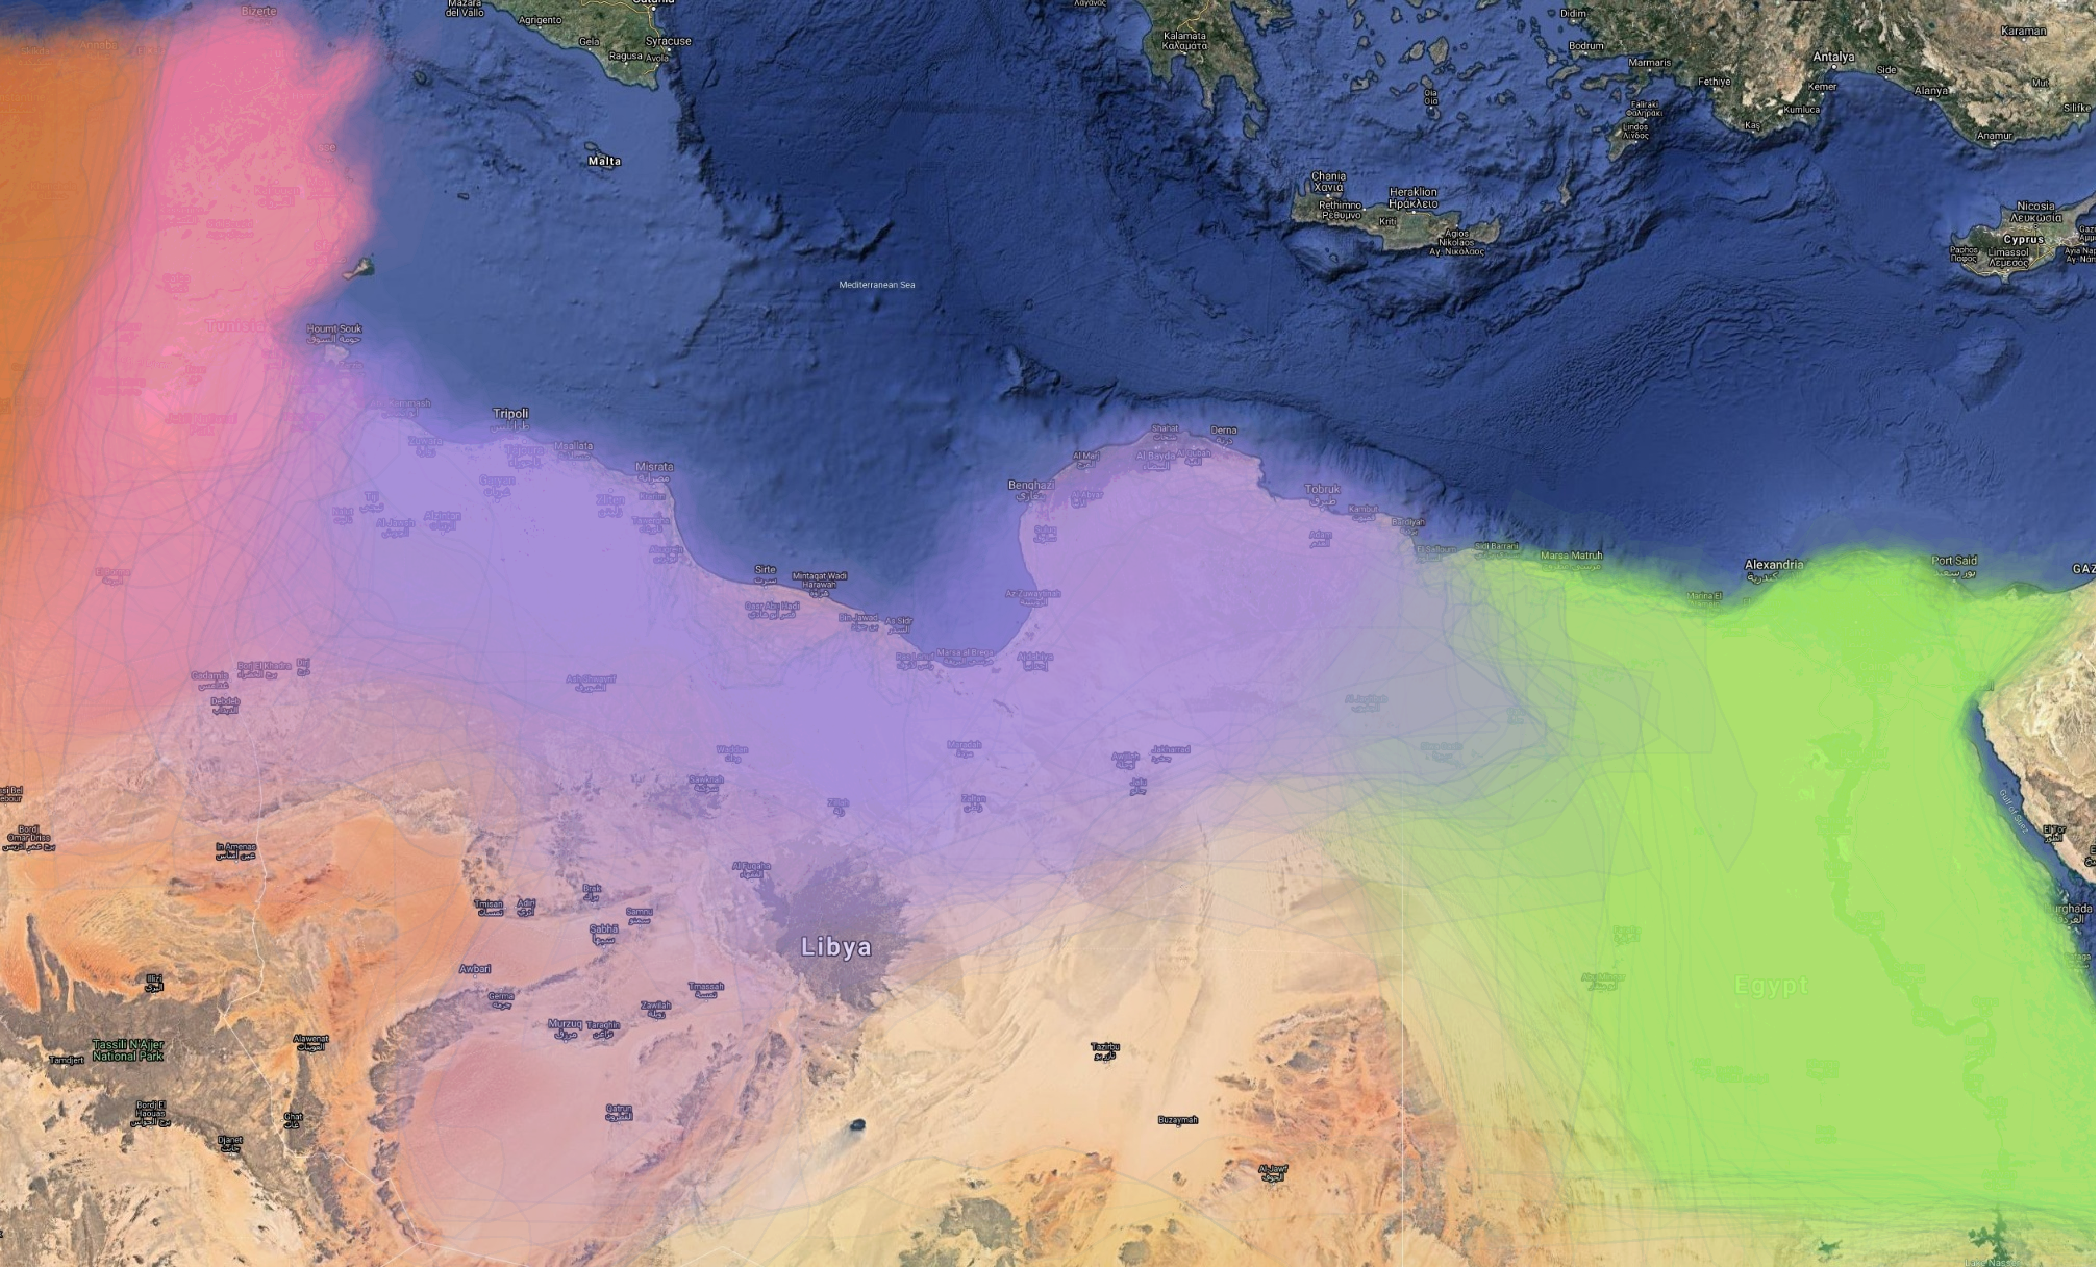
\includegraphics[width=0.8\textwidth,keepaspectratio]{../TUNLIBEGY.pdf}
	\caption{Overlay of all map polygons of Tunisia, Libya and Egypt}
	\label{overlay}
\end{figure}

\begin{multicols}{2}

The data from this project can be aggregated and used in many ways and to
produce many variables. All of these indicators are aggregated over all years
for individual PRIO-GRID cells in Africa. The primary indicator used in this
essay is a measure of the presence of one state over time. It is measured by the
number of maps that indicate that a state was present there, counting only those
of the state most often present in that cell. Figure \ref{Sp} shows the log
transformation (to lessen the visual impact of large variations in the number of
maps for different states) of this measure for all African PRIO grid cells.

\end{multicols}

\begin{figure}[htpb]
	\centering
	%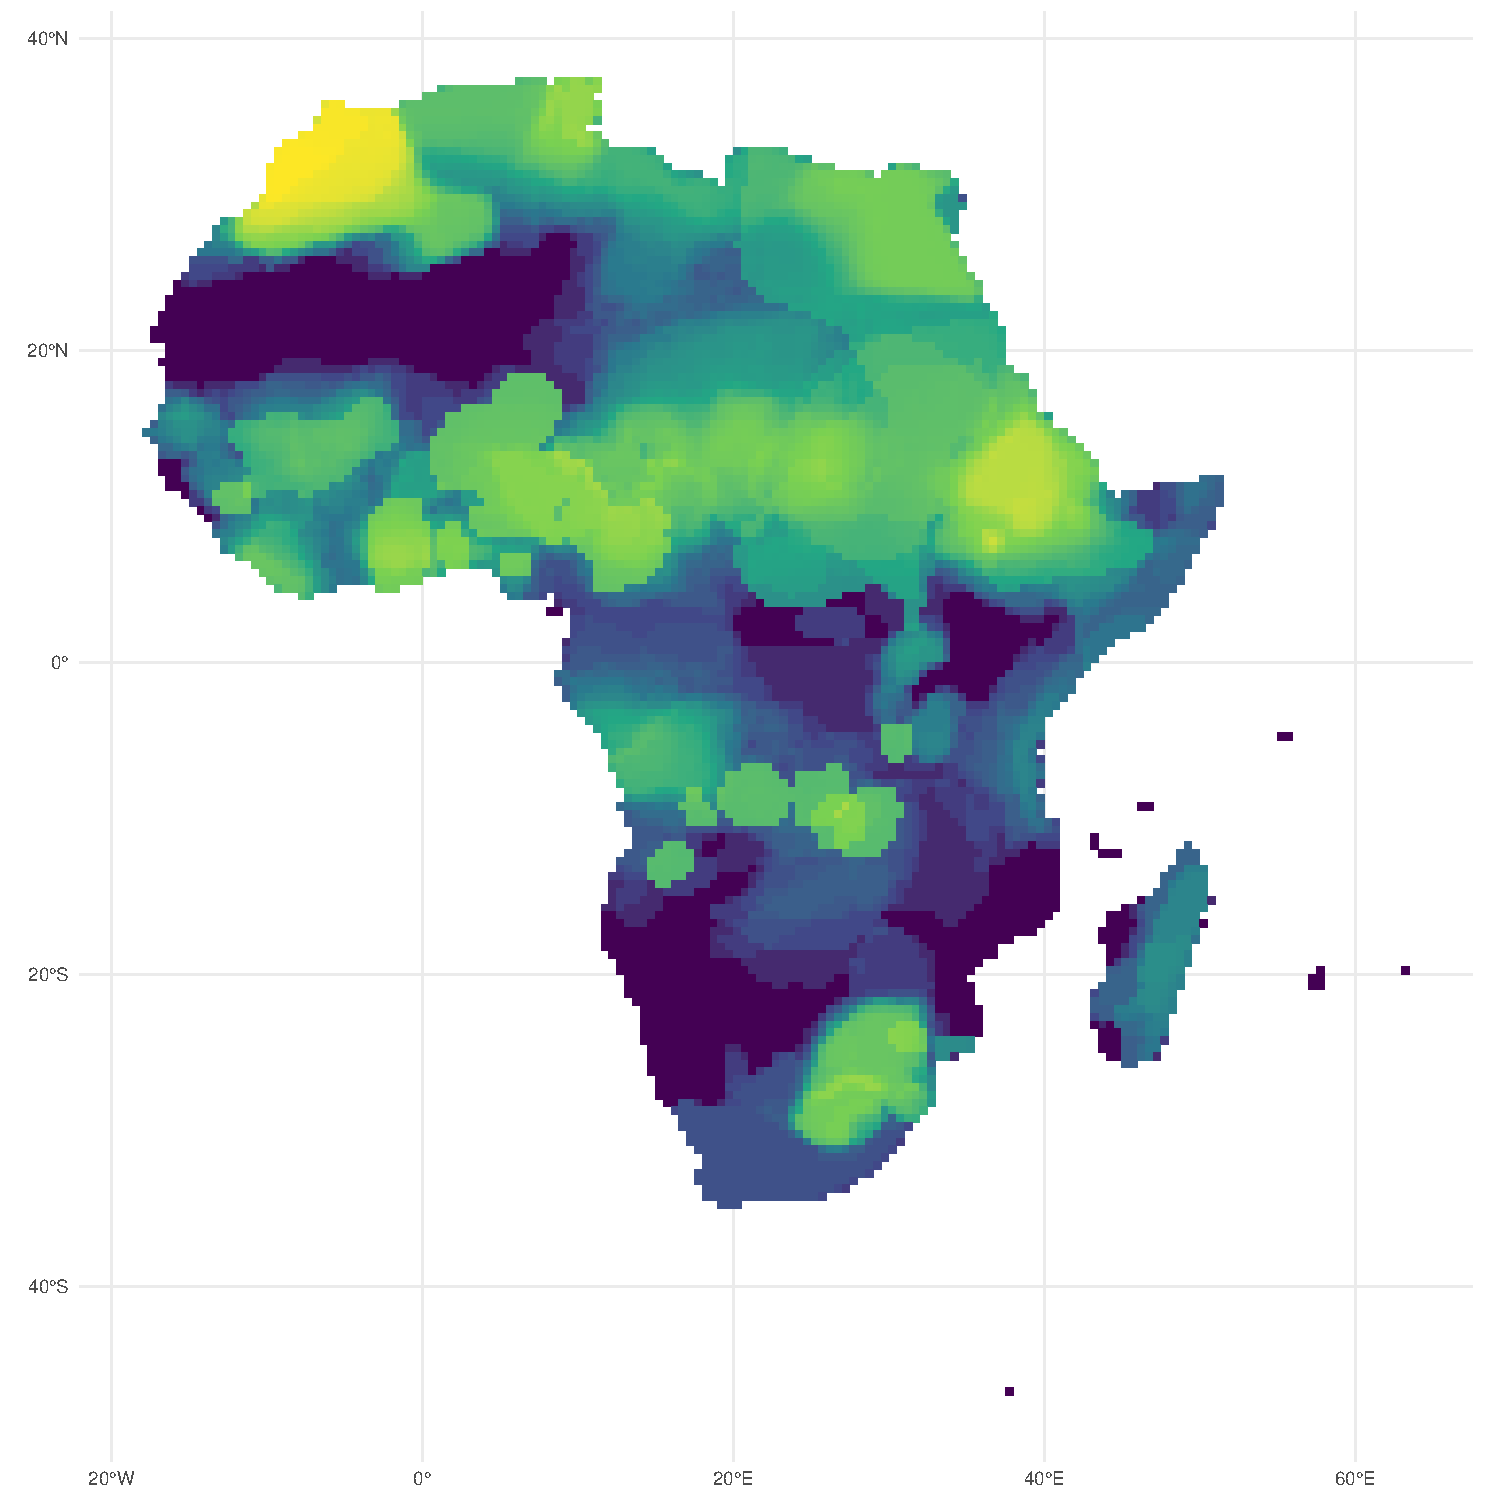
\includegraphics[width=0.8\linewidth]{../Rplot_ln_sp_int.pdf}
	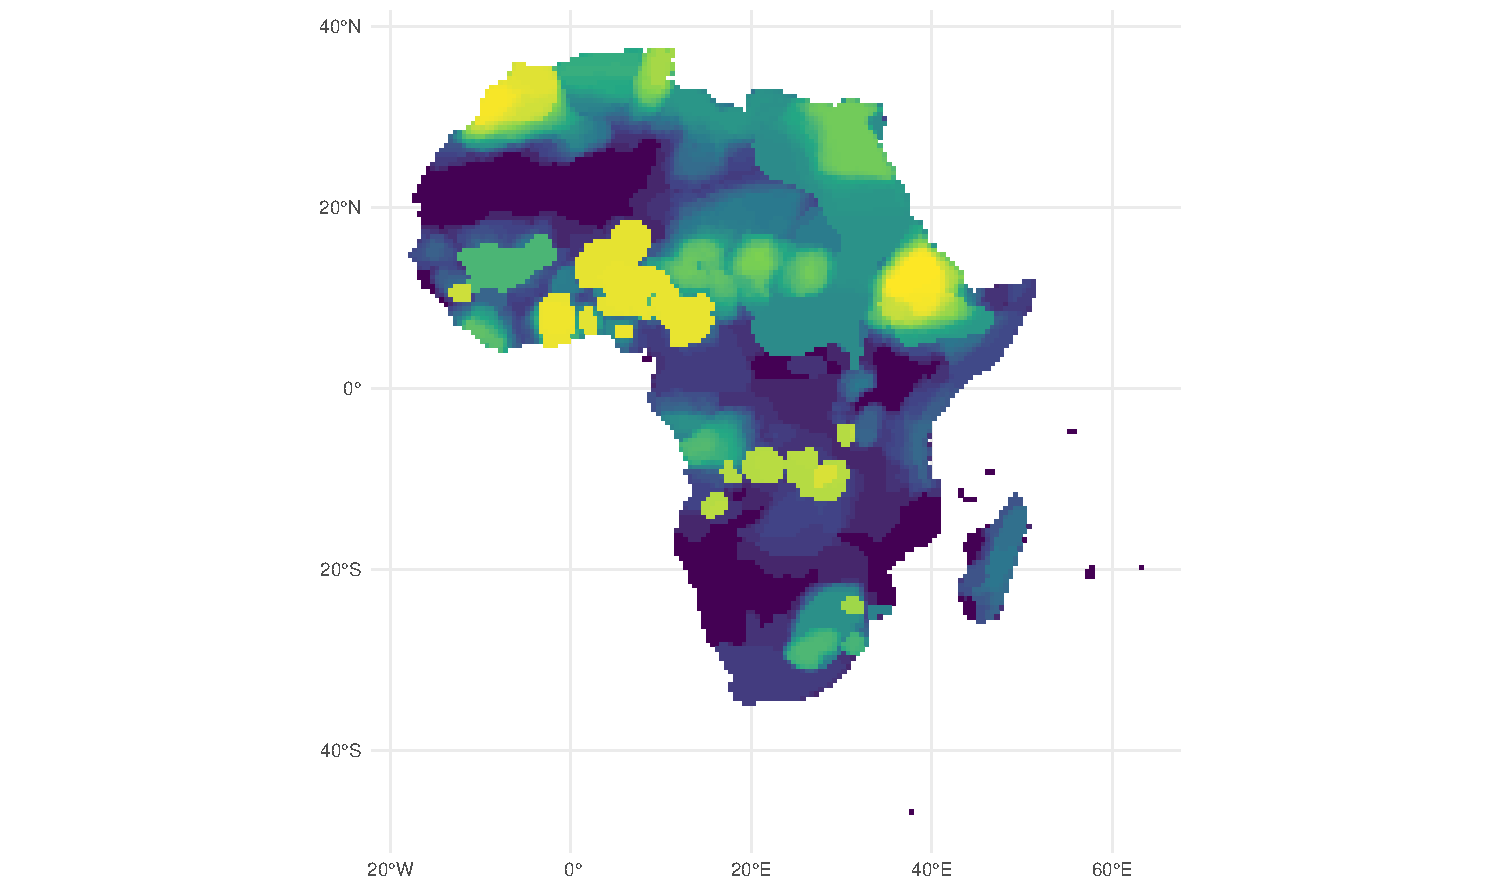
\includegraphics[width=\linewidth]{../R/Output/sp_os_i_sum_any_plot.pdf}
	\caption{State presence (sqrt transformed) with interpolated years based
	on historical atlases.}
	\label{Sp_i}
\end{figure}

\begin{figure}[htpb]
	\centering
	%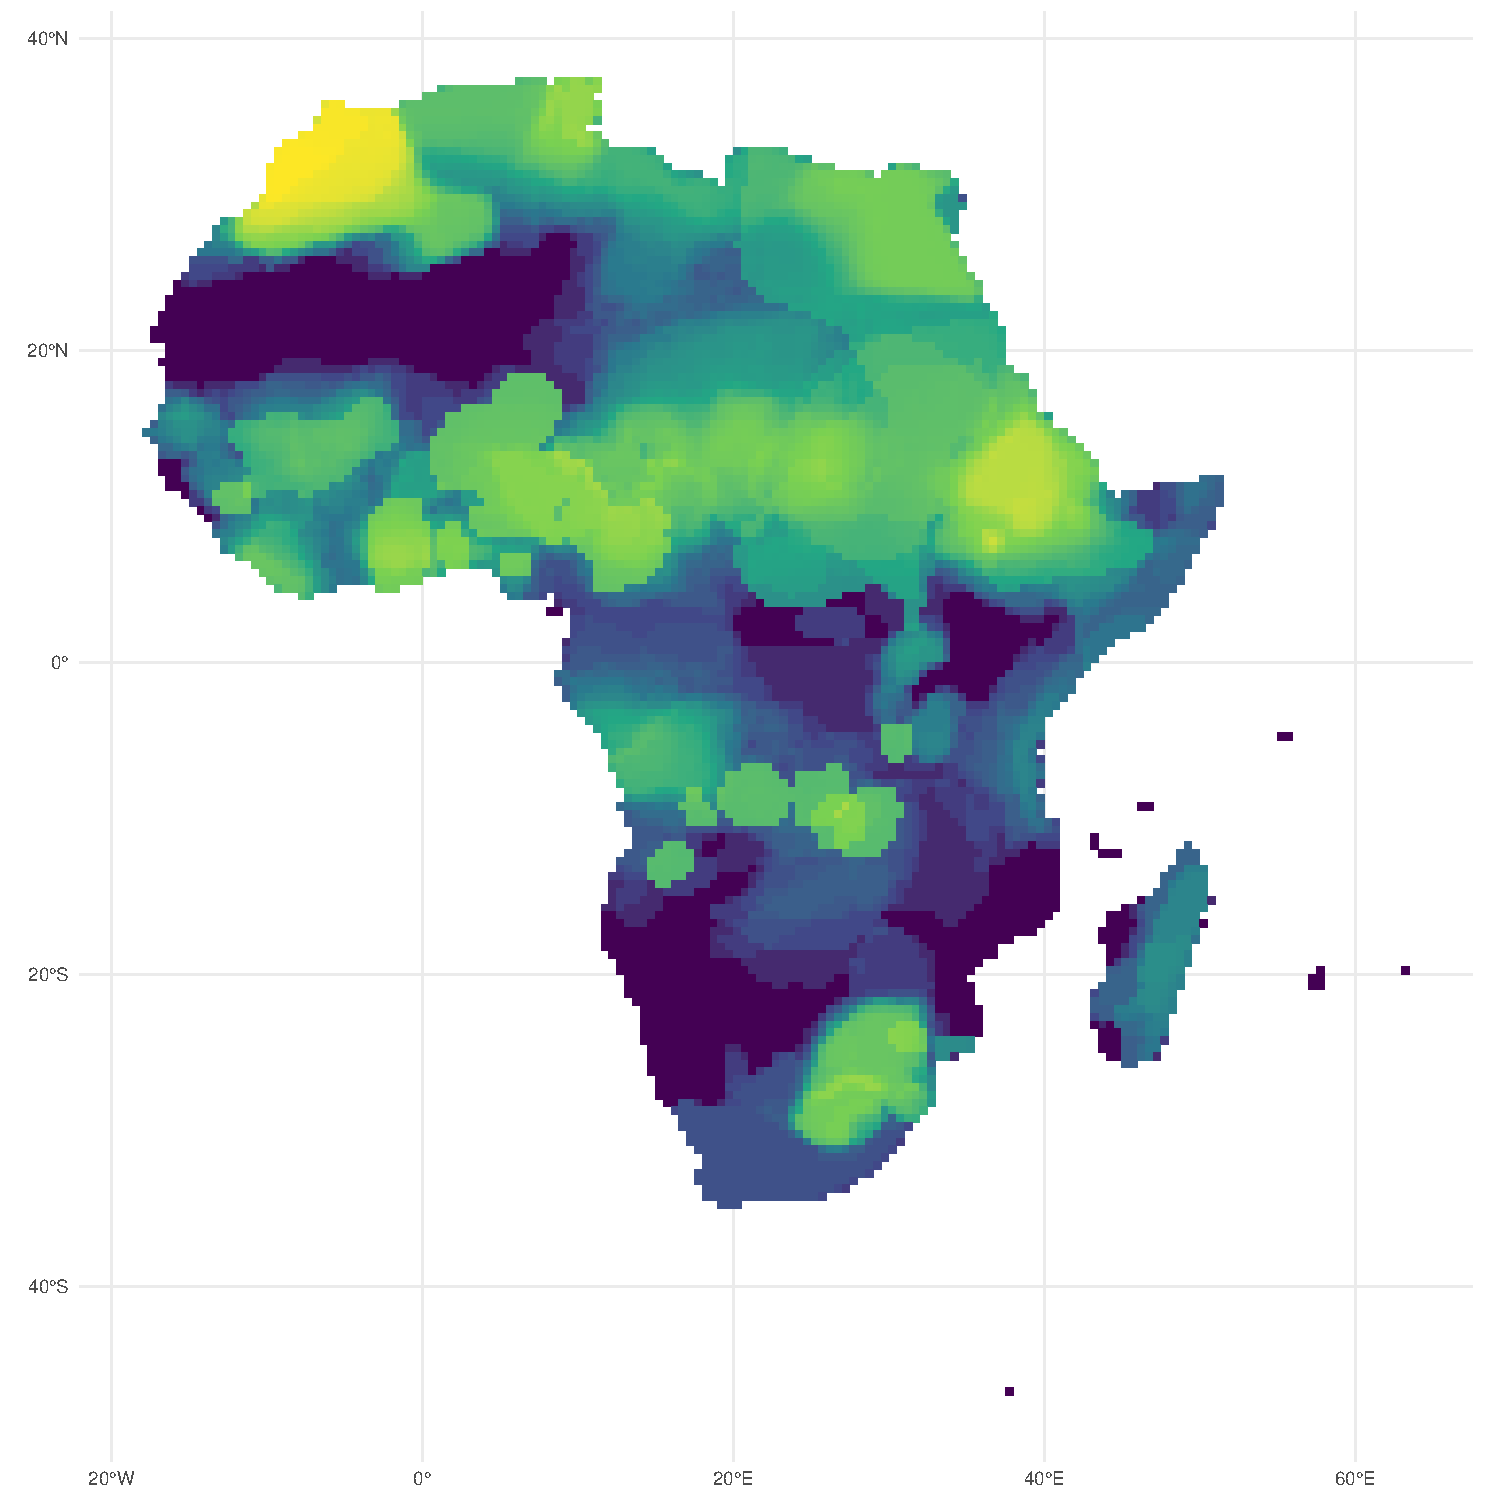
\includegraphics[width=0.8\linewidth]{../Rplot_ln_sp_int.pdf}
	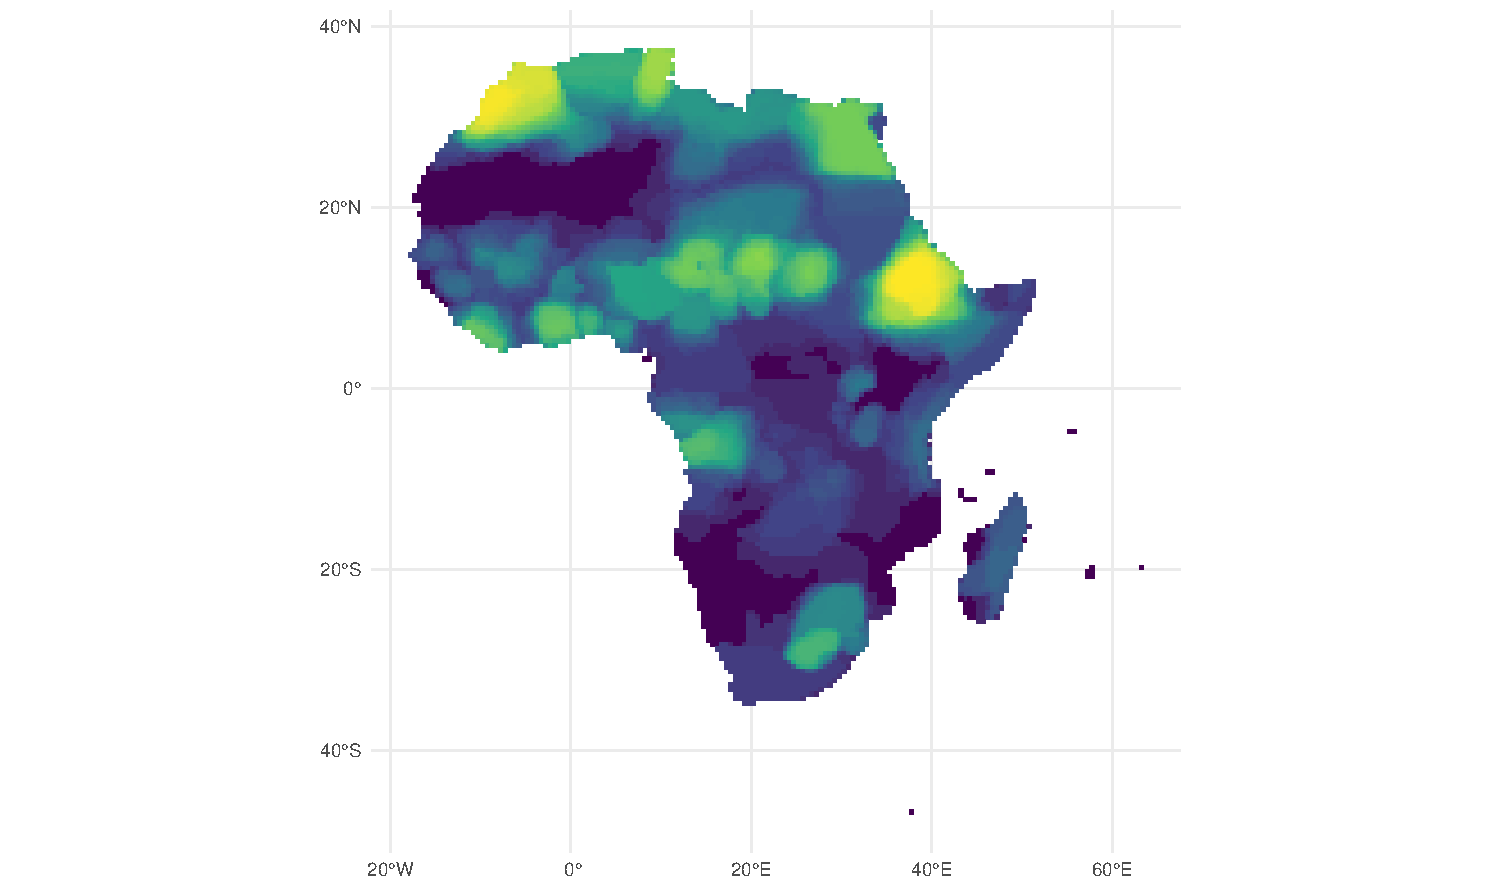
\includegraphics[width=\linewidth]{../R/Output/sp_os_sum_any_plot.pdf}
	\caption{State presence (sqrt transformed)}
	\label{Sp}
\end{figure}

\begin{multicols}{2}

\section{Research design}

\subsection{Dependent variable}

The unit of analysis are PRIO grid cells, which are one degree by one degree
cells \citep{Tollefsen2012}. Accordingly, the dependent variables are fatalities
- square root transformed, logged or untransformed, and state based conflict
events - square root transformed, logged or untransformed) per grid cell in the
period 1946-2018 *** Check end date ***. In other words these are cross
sectional count data. The data are from the GED project \citep{Sundberg2013}.

\subsection{Independent variable}

The main explanatory variable is the per grid cell sum of state presence -
square root transformed or logged depending on the model. For the main model I
use measure of state presence from the Geo-ISD that counts all maps that
intersect a given grid cell, even if multiple maps do so in a single year, but
only for the state that has the most presence overall in that grid cell. This
measure has the benefit of including more data, which allows for the
approximation of relative degrees of state presence by one state in any year, as
described in the data section above. At the same time it avoids over counting
state presence where there were overlaps in sovereignty or changes in who
controlled the territory. As a robustness check I also ran models using the
measure that counts if there was any state presence in a grid-cell-year. In
other words, it is more so a measure of the maximum \textit{extent} of state
presence, and is less accurate in terms of depth. Again counting only the
presence of the most present state for each grid cell.

*** DISCLAIMER - the models reported in the results use this last measure.
However, models using the main measure are very similar. *** 

\subsection{Controls}

Mountains help in early state formation by providing protection and limiting the
exit options of sedentary farmers \citep{Carneiro1988}. Mountainous terrain has
also been linked with civil conflict by providing shelter for rebel groups
\citep{Hegre2006}, although this relationship is debated 
\citep{Buhaug2002}. The data is from the PRIO-grid data set, but originally 
from *** INSERT SOURCE ***.

Water is essential for state formation. States typically formed either as
coastal cities, close to navigable rivers or by the shores of great lakes.
People still tend to live next to a source of water, thus this acts as a proxy
for population density, and fighting usually happens where there are people.
Water could also be related to the conflict measures more directly by being a
non divisible resource to fight for control over. *** SOURCES NEEDED ***. The
data on water as a percentage of the grid surface is from the PRIO-grid data
set, but originally from *** INSERT SOURCE ***.

Distance to coast could affect both state presence and conflict in a number of
ways. First, as state above, states were more likely to be formed along the
coast as it connected cities and people. A special case for Africa is also the
existence of slave raiding/trading states that formed along the eastern and
western coasts of the continent. These states raison d'être was raiding slaves
from tribes and peoples inland and selling them to coastal traders (European in
the West and Arab in the east). \citet{Nunn2008} argues that this state of
affairs left legacies of mistrust and antagonism, which has resulted in
increased levels of current day conflict. Distance to the coast could also be
related to the measure of state presence through the fact that our measure is
based on European observations (maps), which undoubtedly had better coverage
along the coast, especially for the earlier periods. Distance to the coast could
further be related to conflict through lower levels of development. The distance
to coast data is from the PRIO-grid data set, but originally from *** INSERT
SOURCE ***.

Barren terrain could correlate with both state presence and conflict by 

Population density could be a consequence of prior state building and could
correlate with conflit measures as fighting broadly speaking happens where there
are at least some population. I therefor include an estimate of population
density in *** INSERT YEAR *** from the HYDE project \citep{Goldewijk2016}.
Because this is an estimate and not a measurement, I also include a measure of
the barrenness of each grid cell from the PRIO-grid data set, but originally
from *** INSERT SOURCE ***. This measure proxies population density because
people generally do not live on barren land, and captures the large amount of
zeroes in both the Sahara and Kalahari deserts.

As a robustness check some models also include measures of temperature (mean and
variance), precipitation (mean and variance) and forest (remove?), as these have
been found to affect conflict and could potentially affect state building ***
Ask Ole Magnus about these, I don't see the connection ***

Distance to borders *** Put back in ***. Could be related to state presence
because despite their reputation African borders were not drawn completely at
random (or along meridian lines). For example, the borders of northern Nigeria
and Niger were based on the extent of the Sokoto Caliphate and the neighboring
Kanem-Bornu (or just Bornu) empire \citep{HiribarrenVincent2017AHoB}. Proximity
to international border has also been found to predict conflict
\citep{Buhaug2002}. I use the measure included in the PRIO grid data, which is
originally from *** ISERT SOURCE ***.

\subsection{Alternative measures}

*** So far I have none ***

\subsection{Modelling}

My main models are negative binomial models to account for the dependent
variable being count data (count of deaths (fatalities) and count of conflict
events (state based)). *** As I currently understand the assumptions of it, I
should not have to transform the data, as I have done (in the results presented
below), as the negative binomial model accounts for the non-linear nature of the
data. ***

TODO: To fitness test for whether negative binomial or Poisson regression is
most appropriate. I suspected it would be negative binomial, so I went with
that, but this needs to be confirmed.

Zero inflated negative binomial is probably a good idea. Zeros could be true
zeros - there were no fatalities or state based conflict events in the grid cell
during the period, or zeros could be measurement error, most likely resulting
from lack of reporting. However, I am not familiar with ZIMB models at this
point, but I will figure it out before the next draft.

I should also probably be controlling for spatial interdependence, but again, I
am not yet familiar with the method of doing so. Will be addressed in future
versions.

\section{Preliminary results}

I have run a whole lot of model specifications, some of which are reported below
in the figures and in the tables in the appendix. The positive relationship
between state presence and conflict is as surprising as it is robust across all
models. The results of the interaction models might help explain the
relationship. As seen in Figure \ref{deaths_int} and Figure \ref{sb_int}, state
presence is negatively correlated with both conflict measure close to the
capital, but becomes positive and significant further away from the capital.
This supports an interpretation that state presence can be conflict reducing in
those cases where it makes a country less artificial for all the reasons
outlined by the conflict reducing arguments in the literature. Taken tougher
however, the results indicate that the negative effects of higher values of
state presence further away form the capitals of Africa outweighs these conflict
reducing effects. 

\end{multicols}

\begin{figure}[htpb]
	\centering
	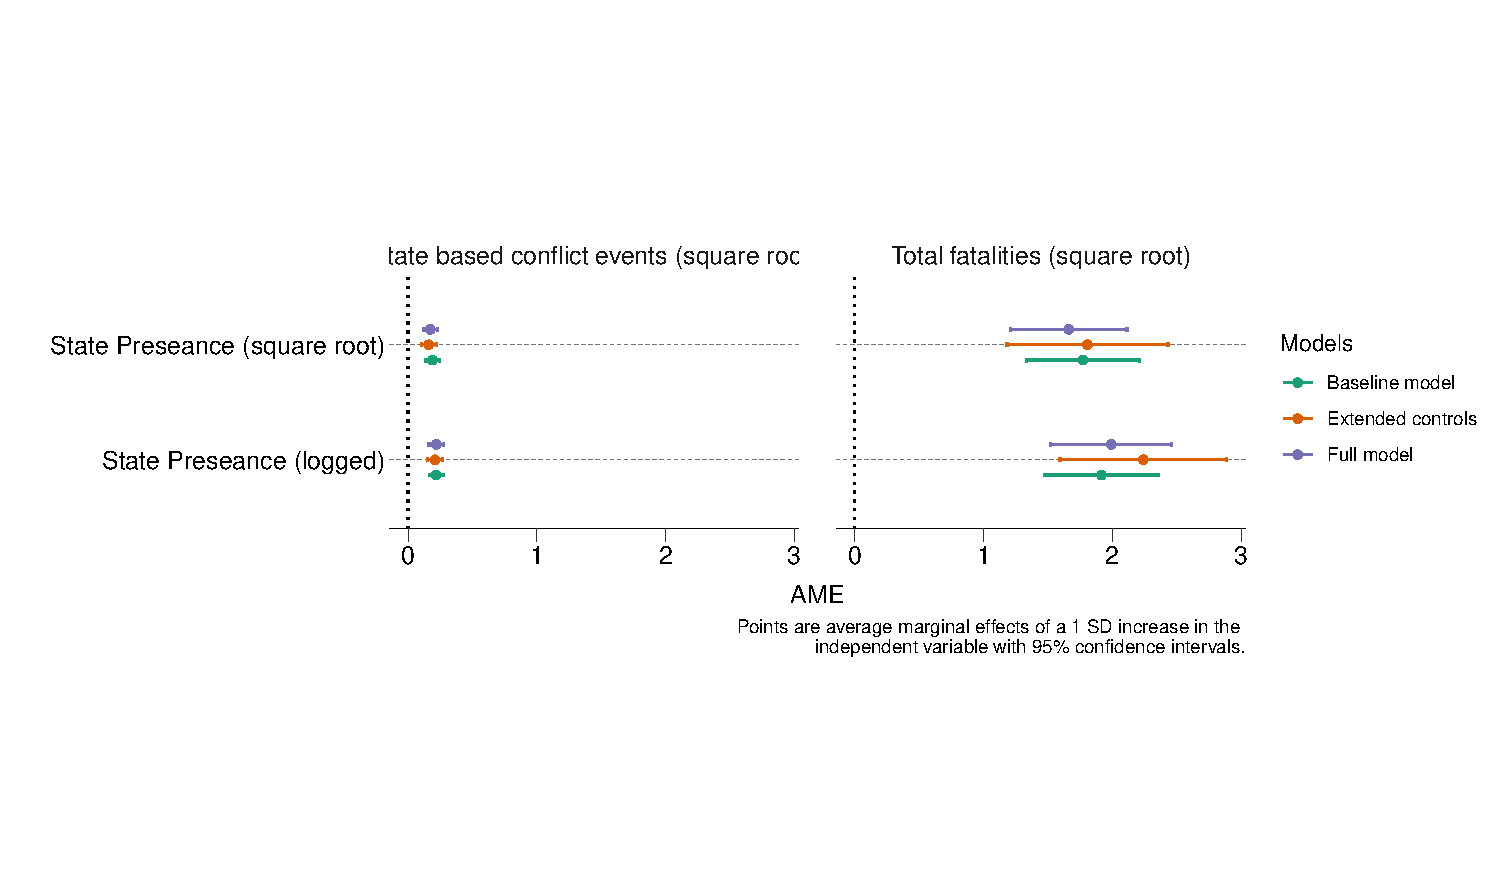
\includegraphics[width=\linewidth]{"../R/Output/conflictMargins.pdf"}
	\caption{}
	\label{margins}
\end{figure}

\begin{figure}[htpb]
	\centering
	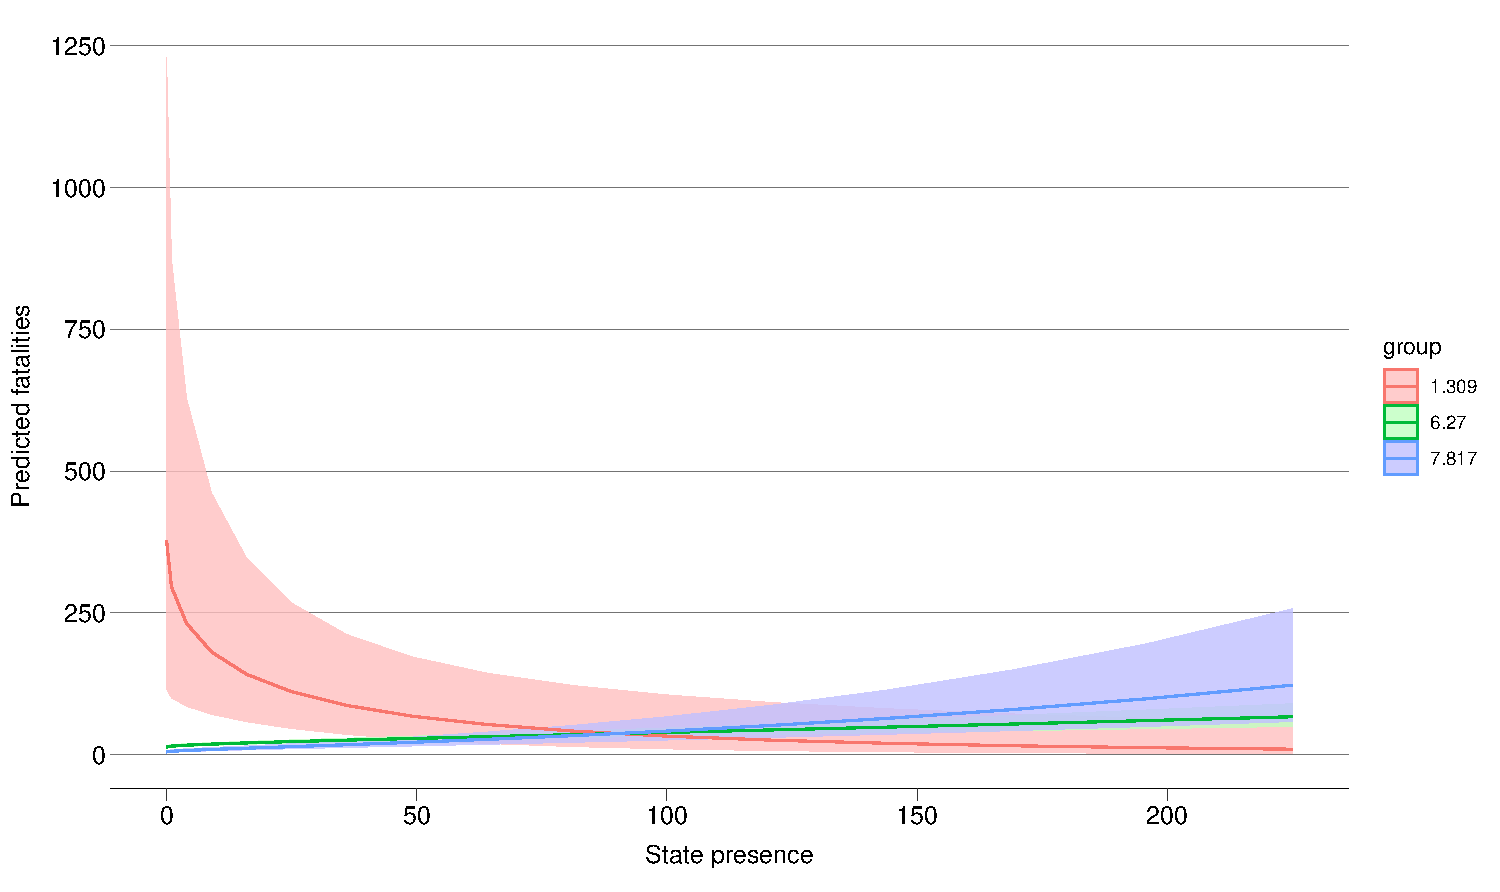
\includegraphics[width=\linewidth]{"../R/Output/deathsIntPlot.pdf"}
	\caption{}
	\label{deaths_int}
\end{figure}

\begin{figure}[htpb]
	\centering
	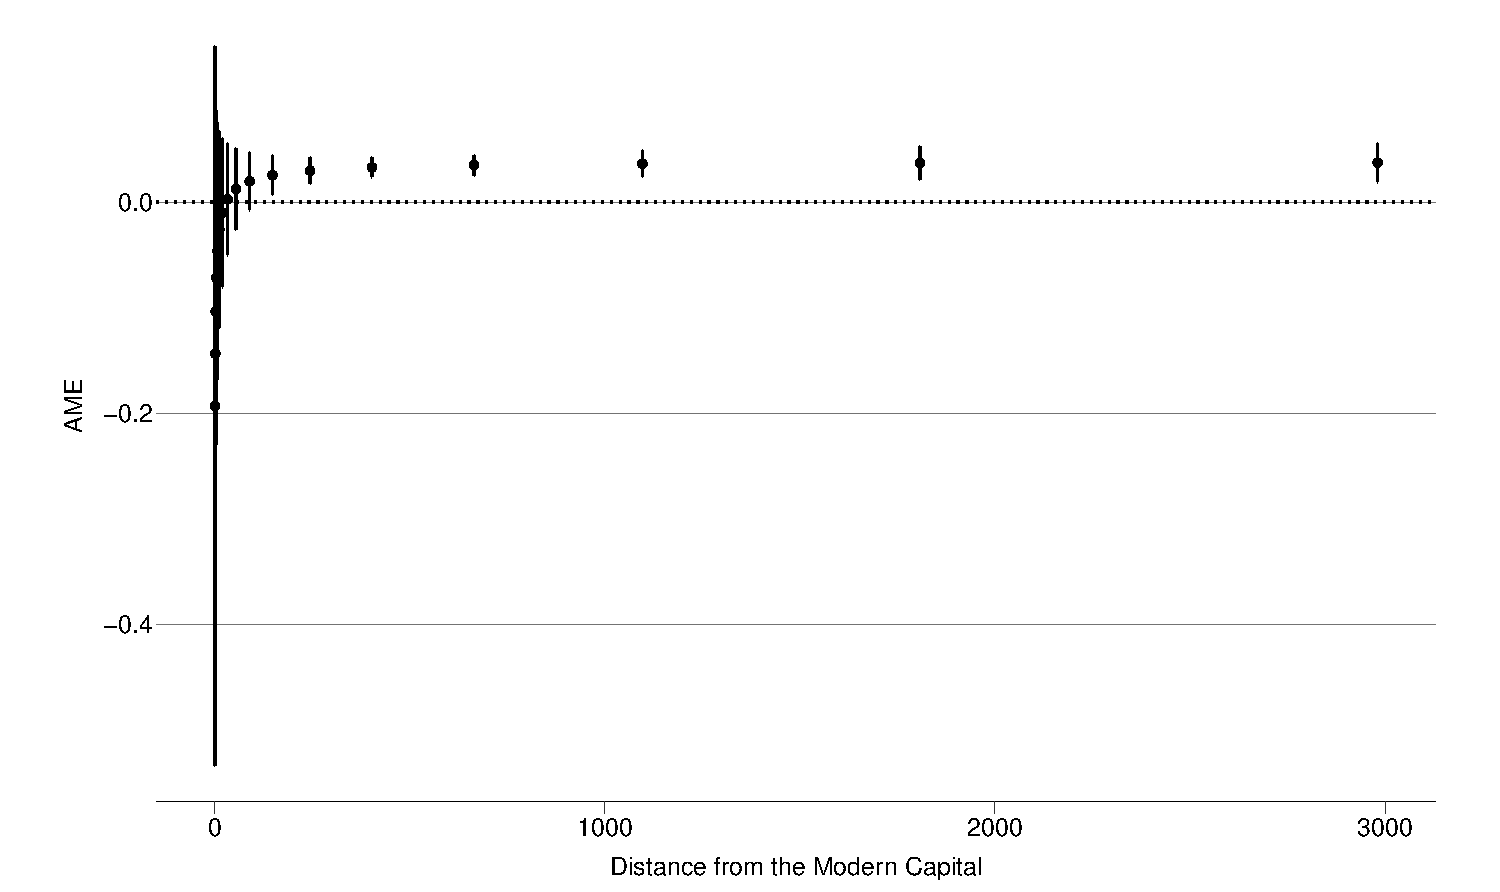
\includegraphics[width=\linewidth]{"../R/Output/state_based_int_plot.pdf"}
	\caption{}
	\label{sb_int}
\end{figure}

\begin{multicols}{2}

\section{Conclusion}

*** Awaiting more detailed results ***

\end{multicols}

\pagebreak

\bibliographystyle{agsm}
\bibliography{../lib.bib}

\pagebreak
\section*{Appendix}


\begin{sidewaystable}
\begin{center}
\scalebox{1}{
\begin{tabular}{l c c c c c c}
\hline
 & Baseline & Extended Controls & Baseline & Extended Controls & Baseline & Extended Controls \\
\hline
(Intercept)     & $3.26^{***}$  & $2.29^{***}$  & $3.65^{***}$  & $2.63^{***}$  & $4.07^{***}$  & $2.95^{***}$  \\
                & $(0.13)$      & $(0.14)$      & $(0.12)$      & $(0.13)$      & $(0.11)$      & $(0.13)$      \\
logSpAll        & $0.30^{***}$  & $0.28^{***}$  &               &               &               &               \\
                & $(0.03)$      & $(0.03)$      &               &               &               &               \\
mountains\_mean & $2.36^{***}$  & $1.24^{***}$  & $2.29^{***}$  & $1.08^{***}$  & $2.21^{***}$  & $1.09^{***}$  \\
                & $(0.19)$      & $(0.19)$      & $(0.19)$      & $(0.19)$      & $(0.20)$      & $(0.19)$      \\
water\_gc       & $0.02^{***}$  & $0.01^{***}$  & $0.03^{***}$  & $0.01^{***}$  & $0.02^{***}$  & $0.01^{***}$  \\
                & $(0.00)$      & $(0.00)$      & $(0.00)$      & $(0.00)$      & $(0.00)$      & $(0.00)$      \\
barren\_gc      & $-0.03^{***}$ & $-0.02^{***}$ & $-0.03^{***}$ & $-0.02^{***}$ & $-0.03^{***}$ & $-0.02^{***}$ \\
                & $(0.00)$      & $(0.00)$      & $(0.00)$      & $(0.00)$      & $(0.00)$      & $(0.00)$      \\
distcoast       & $0.00^{***}$  & $0.00^{***}$  & $0.00^{***}$  & $0.00^{***}$  & $0.00^{***}$  & $0.00^{***}$  \\
                & $(0.00)$      & $(0.00)$      & $(0.00)$      & $(0.00)$      & $(0.00)$      & $(0.00)$      \\
logPopd         &               & $1.03^{***}$  &               & $1.03^{***}$  &               & $1.05^{***}$  \\
                &               & $(0.07)$      &               & $(0.07)$      &               & $(0.07)$      \\
bdist3          &               & $-0.00^{*}$   &               & $-0.00^{*}$   &               & $-0.00^{*}$   \\
                &               & $(0.00)$      &               & $(0.00)$      &               & $(0.00)$      \\
sqrtSpAll       &               &               & $0.10^{***}$  & $0.09^{***}$  &               &               \\
                &               &               & $(0.01)$      & $(0.01)$      &               &               \\
SpAll10         &               &               &               &               & $0.00^{***}$  & $0.00^{***}$  \\
                &               &               &               &               & $(0.00)$      & $(0.00)$      \\
\hline
AIC             & $43066.10$    & $42817.43$    & $43101.68$    & $42851.53$    & $43143.35$    & $42890.13$    \\
BIC             & $43116.91$    & $42882.75$    & $43152.48$    & $42916.85$    & $43194.16$    & $42955.45$    \\
Log Likelihood  & $-21526.05$   & $-21399.71$   & $-21543.84$   & $-21416.77$   & $-21564.67$   & $-21436.07$   \\
Deviance        & $5340.87$     & $5355.31$     & $5338.89$     & $5353.37$     & $5336.65$     & $5351.13$     \\
Num. obs.       & $10492$       & $10482$       & $10492$       & $10482$       & $10492$       & $10482$       \\
\hline
\multicolumn{7}{l}{\scriptsize{$^{***}p<0.001$; $^{**}p<0.01$; $^{*}p<0.05$; $^{\cdot}p<0.1$}}
\end{tabular}
}
\caption{Fatalities}
\label{deaths}
\end{center}
\end{sidewaystable}


\begin{sidewaystable}
\begin{center}
\scalebox{1}{
\begin{tabular}{l c c c c}
\toprule
 & Geography & North Africa & Population densisty & Distance
		  to border \\
\midrule
Precolonial state presence (sqrt)        & $0.07^{***}$  & $0.05^{***}$  & $0.04^{***}$  & $0.04^{***}$    \\
                                         & $(0.01)$      & $(0.01)$      & $(0.01)$      & $(0.01)$        \\
Precolonial state presence (sqrt)        & $0.07^{***}$  & $0.05^{***}$  & $0.04^{***}$  & $0.04^{***}$    \\
                                         & $(0.01)$      & $(0.01)$      & $(0.01)$      & $(0.01)$        \\
Mountainous terrain                      & $0.87^{***}$  & $0.81^{***}$  & $-0.22$       & $-0.28^{\cdot}$ \\
                                         & $(0.16)$      & $(0.16)$      & $(0.15)$      & $(0.15)$        \\
Water (\%)                               & $-0.01^{*}$   & $-0.01^{*}$   & $-0.01^{**}$  & $-0.01^{***}$   \\
                                         & $(0.00)$      & $(0.00)$      & $(0.00)$      & $(0.00)$        \\
Barren (\%)                              & $-0.02^{***}$ & $-0.02^{***}$ & $-0.01^{***}$ & $-0.01^{***}$   \\
                                         & $(0.00)$      & $(0.00)$      & $(0.00)$      & $(0.00)$        \\
Distance to coast (log)                  & $-0.16^{***}$ & $-0.14^{***}$ & $-0.11^{***}$ & $-0.08^{***}$   \\
                                         & $(0.02)$      & $(0.02)$      & $(0.02)$      & $(0.02)$        \\
Population density (log)                 &               &               & $1.00^{***}$  & $0.94^{***}$    \\
                                         &               &               & $(0.06)$      & $(0.06)$        \\
Distance to international boundary (log) &               &               &               & $-0.20^{***}$   \\
                                         &               &               &               & $(0.04)$        \\
North Africa                             &               & $0.51^{***}$  & $0.38^{**}$   & $0.47^{***}$    \\
                                         &               & $(0.13)$      & $(0.12)$      & $(0.12)$        \\
\midrule
AIC                                      & $20314.22$    & $20297.34$    & $20007.10$    & $19979.16$      \\
BIC                                      & $20364.33$    & $20354.61$    & $20071.52$    & $20050.74$      \\
Log Likelihood                           & $-10150.11$   & $-10140.67$   & $-9994.55$    & $-9979.58$      \\
Deviance                                 & $4106.74$     & $4112.96$     & $4158.66$     & $4164.26$       \\
Num. obs.                                & $9492$        & $9492$        & $9492$        & $9492$          \\
\bottomrule
\multicolumn{5}{l}{\scriptsize{$^{***}p<0.001$; $^{**}p<0.01$; $^{*}p<0.05$; $^{\cdot}p<0.1$}}
\end{tabular}
}
\caption{State based conflict events}
\label{state_based}
\end{center}
\end{sidewaystable}


\begin{sidewaystable}
\begin{center}
\scalebox{1}{
\begin{tabular}{l c c c}
\hline
 & Baseline & Extetended Controls & Full Model \\
\hline
(Intercept)          & $2.84^{***}$   & $1.93^{***}$  & $-0.82$       \\
                     & $(0.45)$       & $(0.45)$      & $(0.52)$      \\
sqrtSpAny            & $-0.06$        & $-0.36^{***}$ & $-0.30^{***}$ \\
                     & $(0.09)$       & $(0.09)$      & $(0.08)$      \\
logCapdist           & $-0.39^{***}$  & $-0.35^{***}$ & $-0.33^{***}$ \\
                     & $(0.07)$       & $(0.07)$      & $(0.07)$      \\
mountains\_mean      & $1.04^{***}$   & $0.65^{***}$  & $1.03^{***}$  \\
                     & $(0.13)$       & $(0.12)$      & $(0.13)$      \\
water\_gc            & $0.01^{***}$   & $0.01^{***}$  & $0.01^{***}$  \\
                     & $(0.00)$       & $(0.00)$      & $(0.00)$      \\
barren\_gc           & $-0.02^{***}$  & $-0.01^{***}$ & $-0.01^{***}$ \\
                     & $(0.00)$       & $(0.00)$      & $(0.00)$      \\
distcoast            & $0.00^{***}$   & $0.00^{***}$  & $0.00^{***}$  \\
                     & $(0.00)$       & $(0.00)$      & $(0.00)$      \\
sqrtSpAny:logCapdist & $0.03^{\cdot}$ & $0.07^{***}$  & $0.06^{***}$  \\
                     & $(0.01)$       & $(0.01)$      & $(0.01)$      \\
logPopd              &                & $0.79^{***}$  & $0.82^{***}$  \\
                     &                & $(0.05)$      & $(0.05)$      \\
temp\_sd             &                &               & $0.86^{***}$  \\
                     &                &               & $(0.10)$      \\
temp                 &                &               & $0.05^{***}$  \\
                     &                &               & $(0.01)$      \\
prec\_sd             &                &               & $0.00$        \\
                     &                &               & $(0.00)$      \\
prec\_gpcc           &                &               & $0.00^{*}$    \\
                     &                &               & $(0.00)$      \\
forest\_gc           &                &               & $0.00$        \\
                     &                &               & $(0.00)$      \\
\hline
AIC                  & $29512.34$     & $29259.38$    & $29035.25$    \\
BIC                  & $29577.67$     & $29331.95$    & $29144.07$    \\
Log Likelihood       & $-14747.17$    & $-14619.69$   & $-14502.63$   \\
Deviance             & $5713.62$      & $5758.34$     & $5778.58$     \\
Num. obs.            & $10492$        & $10482$       & $10453$       \\
\hline
\multicolumn{4}{l}{\scriptsize{$^{***}p<0.001$; $^{**}p<0.01$; $^{*}p<0.05$; $^{\cdot}p<0.1$}}
\end{tabular}
}
\caption{Deaths * Distance to capital}
\label{interaction_sqrtDeaths}
\end{center}
\end{sidewaystable}


\begin{sidewaystable}
\begin{center}
\scalebox{1}{
\begin{tabular}{l c c c}
\hline
 & Baseline & Extetended Controls & Full Model \\
\hline
(Intercept)          & $0.91^{*}$    & $-0.50$        & $-3.62^{***}$   \\
                     & $(0.40)$      & $(0.39)$       & $(0.47)$        \\
sqrtSpAny            & $-0.04$       & $-0.24^{**}$   & $-0.09$         \\
                     & $(0.07)$      & $(0.07)$       & $(0.07)$        \\
logCapdist           & $-0.33^{***}$ & $-0.18^{**}$   & $-0.12^{\cdot}$ \\
                     & $(0.06)$      & $(0.06)$       & $(0.06)$        \\
mountains\_mean      & $0.58^{***}$  & $0.19^{\cdot}$ & $0.65^{***}$    \\
                     & $(0.11)$      & $(0.11)$       & $(0.12)$        \\
water\_gc            & $0.01^{**}$   & $0.00^{\cdot}$ & $0.01^{**}$     \\
                     & $(0.00)$      & $(0.00)$       & $(0.00)$        \\
barren\_gc           & $-0.01^{***}$ & $-0.01^{***}$  & $-0.01^{***}$   \\
                     & $(0.00)$      & $(0.00)$       & $(0.00)$        \\
distcoast            & $0.00^{**}$   & $0.00$         & $0.00^{*}$      \\
                     & $(0.00)$      & $(0.00)$       & $(0.00)$        \\
sqrtSpAny:logCapdist & $0.02$        & $0.05^{***}$   & $0.02^{*}$      \\
                     & $(0.01)$      & $(0.01)$       & $(0.01)$        \\
logPopd              &               & $0.70^{***}$   & $0.79^{***}$    \\
                     &               & $(0.04)$       & $(0.04)$        \\
temp\_sd             &               &                & $0.93^{***}$    \\
                     &               &                & $(0.08)$        \\
temp                 &               &                & $0.06^{***}$    \\
                     &               &                & $(0.01)$        \\
prec\_sd             &               &                & $0.01^{**}$     \\
                     &               &                & $(0.00)$        \\
prec\_gpcc           &               &                & $-0.00$         \\
                     &               &                & $(0.00)$        \\
forest\_gc           &               &                & $0.00$          \\
                     &               &                & $(0.00)$        \\
\hline
AIC                  & $15400.86$    & $15138.19$     & $14812.98$      \\
BIC                  & $15466.18$    & $15210.77$     & $14921.80$      \\
Log Likelihood       & $-7691.43$    & $-7559.10$     & $-7391.49$      \\
Deviance             & $4787.30$     & $4853.39$      & $4917.84$       \\
Num. obs.            & $10492$       & $10482$        & $10453$         \\
\hline
\multicolumn{4}{l}{\scriptsize{$^{***}p<0.001$; $^{**}p<0.01$; $^{*}p<0.05$; $^{\cdot}p<0.1$}}
\end{tabular}
}
\caption{State based conflict events *
		  distance to capital}
\label{interaction_sqrtState_based}
\end{center}
\end{sidewaystable}


\end{document}

